\documentclass{standalone}
\usepackage{tikz}
\usetikzlibrary{calc, fit}

\newcommand{\gaussian}[3]{
    % #1: x
    % #2: y
    % #3: color
    \node[cell] (cell0) at (#1,#2) [fill=#3, opacity=0.5] {};
    \node[cell] (cell1) at ($(cell0.south west)-(0.5,0)$) [fill=#3!30, opacity=0.5] {};
    \node[cell] (cell1) at ($(cell0.south west)+(0.5,0)$) [fill=#3!30, opacity=0.5] {};
    \node[cell] (cell1) at ($(cell0.south west)+(0,0.5)$) [fill=#3!30, opacity=0.5] {};
    \node[cell] (cell1) at ($(cell0.south west)-(0,0.5)$) [fill=#3!30, opacity=0.5] {};
    \node[cell] (cell1) at ($(cell0.south west)-(0.5,0.5)$) [fill=#3!10, opacity=0.5] {};
    \node[cell] (cell1) at ($(cell0.south west)+(0.5,0.5)$) [fill=#3!10, opacity=0.5] {};
    \node[cell] (cell1) at ($(cell0.south west)+(-0.5,0.5)$) [fill=#3!10, opacity=0.5] {};
    \node[cell] (cell1) at ($(cell0.south west)+(0.5,-0.5)$) [fill=#3!10, opacity=0.5] {};
}
\newcommand{\grid}{
    \fill[white, fill opacity=.8](-1,-1.5) rectangle (2.5,2.5);
    \draw[step=5mm, gray](-1,-1.5) grid (2.5,2.5);
}

\begin{document}
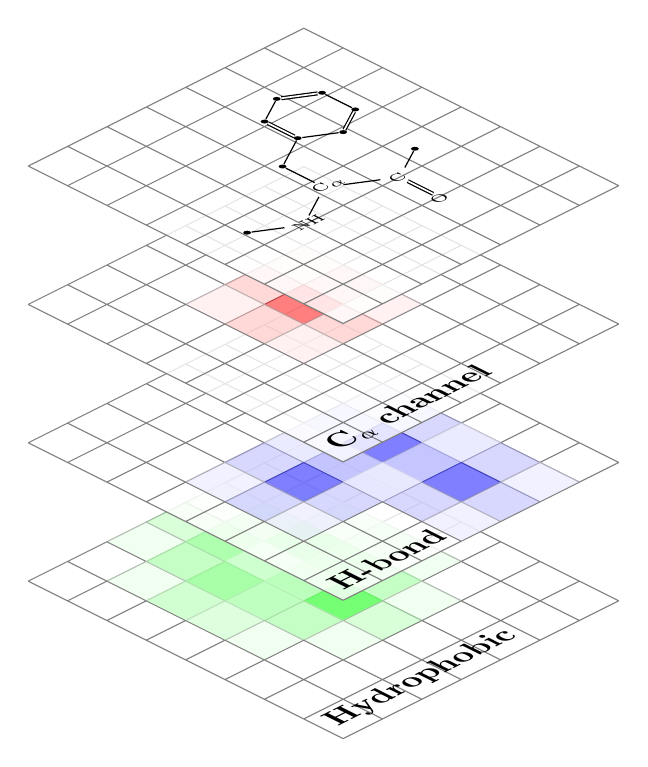
\begin{tikzpicture}
    % implicit atoms (C)
    \tikzstyle{imp}=[inner sep=0, circle, fill=black,minimum size=0.2em]
    % explicit atoms with name
    \tikzstyle{exp}=[inner sep=1, font=\tiny, text width=1.5ex]
    \tikzstyle{cell}=[minimum width=5mm,minimum height=5mm, anchor=south west]
    %  Grid for COB channel
    \begin{scope}[yshift=-150, every node/.append style={yslant=0.5,xslant=-1.},yslant=0.5,xslant=-1.]
        \grid
        \gaussian{0}{.5}{green};
        \gaussian{0}{1.}{green};
        \gaussian{0.5}{1.5}{green};
        \gaussian{1.}{1}{green};
        \gaussian{1.}{.5}{green};
        \gaussian{0.5}{0}{green};
        \node[anchor=south west, font=\bfseries] at (-1,-1.5) {Hydrophobic};
    \end{scope}
        % Grid for HAD channel
    \begin{scope}[yshift=-100, every node/.append style={yslant=0.5,xslant=-1.},yslant=0.5,xslant=-1.]
        \grid
        \gaussian{0}{0}{blue};
        \gaussian{1}{0}{blue};
        \gaussian{1}{-1}{blue};
        \node[anchor=south west, font=\bfseries] at (-1,-1.5) {H-bond};
    \end{scope}
    % Grid for CA channel
    \begin{scope}[yshift=-50, every node/.append style={yslant=0.5,xslant=-1.},yslant=0.5,xslant=-1.]
        \grid
        \gaussian{0.5}{0.5}{red};
        \node[anchor=south west, font=\bfseries] at (-1,-1.5) {C$_{\alpha}$ channel};
    \end{scope}
    \begin{scope}[every node/.append style={yslant=0.5,xslant=-1.},yslant=0.5,xslant=-1.]
        \grid
        \node[exp] (NH) at (0,0) {NH};
        \node[exp] (CA) at ($(NH)+(30:2em)$) {C$_{\alpha}$};
        \node[exp] (CO) at ($(CA)+(-30:2em)$) {C};
        \node[exp] (O) at ($(CO)+(90:-1.5em)$) {O};
        \node[imp] (CB) at ($(CA)+(90:1.5em)$) {};
        \node[imp] (CG) at ($(CB)+(30:1.5em)$) {};
        \node[imp] (CD1) at ($(CG)+(160-70:1.2em)$) {};
        \node[imp] (CE1) at ($(CD1)+(100-70:1.2em)$) {};
        \node[imp] (CZ) at ($(CE1)+(40-70:1.2em)$) {};
        \node[imp] (CE2) at ($(CZ)+(-20-70:1.2em)$) {};
        \node[imp] (CD2) at ($(CE2)+(-80-70:1.2em)$) {};
        \node[imp] (DUM0) at ($(NH)+(-30:-1.5em)$) {};
        \node[imp] (DUM1) at ($(CO)+(30:1.5em)$) {};
        \draw[line width=.1ex] (DUM0) -- (NH) -- (CA) -- (CO) -- (DUM1);
        \draw[line width=.1ex, double] (CO) -- (O);
        \draw[line width=.1ex] (CA) -- (CB);
        \draw[line width=.1ex] (CB) -- (CG);
        \draw[line width=.1ex, double] (CG) -- (CD1);
        \draw[line width=.1ex] (CD1) -- (CE1);
        \draw[line width=.1ex, double] (CE1) -- (CZ);
        \draw[line width=.1ex] (CZ) -- (CE2);
        \draw[line width=.1ex, double] (CE2) -- (CD2);
        \draw[line width=.1ex] (CD2) -- (CG);
        % \node[fit=(NH)(CA)(CO)(O)(CB)(CG)(CD1)(CE1)(CZ)(CE2)(CD2)(DUM0)(DUM1), draw, inner sep=5ex] {};
    \end{scope}
\end{tikzpicture}
\end{document}

